\documentclass[french]{article}
\usepackage[T1]{fontenc}
\usepackage[utf8]{inputenc}
\usepackage{lmodern}
\usepackage[a4paper]{geometry}
\usepackage{babel}
\usepackage{graphicx}

\begin{document}
\title{Nuages de points et modélisation 3D\\
TP 1 : Opérations de bases et structures sur les nuages de points}
\author{Marius Dufraisse}
\date{}

\maketitle


\paragraph{Question 1.} Le résultat de la transformation est présenté Figure \ref{fig:q1}.
\begin{figure}[h]
	\centering
	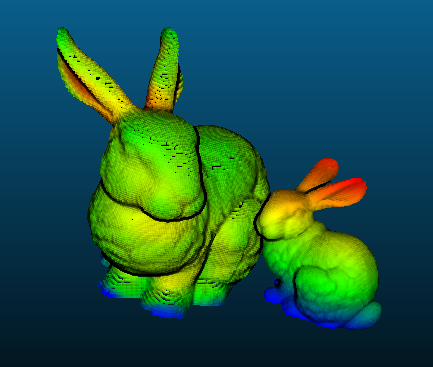
\includegraphics[width=0.55\linewidth]{q1}
	\caption{Le lapin transformé à côté du lapin initial.}
	\label{fig:q1}
\end{figure}

\paragraph{Question 2.} Pour 10 recherches, trouver les $k$ plus proches voisins a pris 0.73 secondes et les les voisins dans un rayon de 20cm a pris 0.70 secondes. Pour calculer les plus proches voisins pour tout le nuage, les deux méthodes auraient pris respectivement 62 et 59 heures.

\paragraph{Question 3.} The optimal leaf size seems to be around 30 (see Figure \ref{fig:leafsize}). Prendre des feuilles de  taille 1 n'est pas optimal car lorsque les feuilles sont suffisamment petites ils est plus efficaces de les parcourir plutôt que de continuer à faire des appels de fonctions récursifs. Par ailleurs on cherche toujours plus d'un seul voisin donc on doit nécessairement explorer des feuilles adjacentes.

\begin{figure}[h]
	\centering
	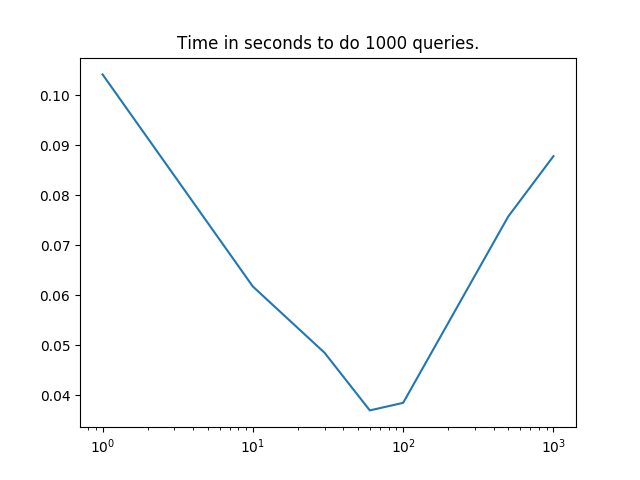
\includegraphics[width=0.6\linewidth]{kdt_lfsize.png}
	\caption{Évolution du temps nécessaire à 1000 recherches en fonction de la taille des feuilles.}
	\label{fig:leafsize}
\end{figure}

\paragraph{Question 4.}
La Figure \ref{fig:radius} montre l'évolution du temps nécessaire pour réaliser 1000 recherches en fonction du rayon. Plus le rayon est grand, plus la recherche prends du temps. En utilisant des kdtree faire une recherche à 20cm pour tous les points ne prendrait que 3 minutes.


\begin{figure}[h]
	\centering
	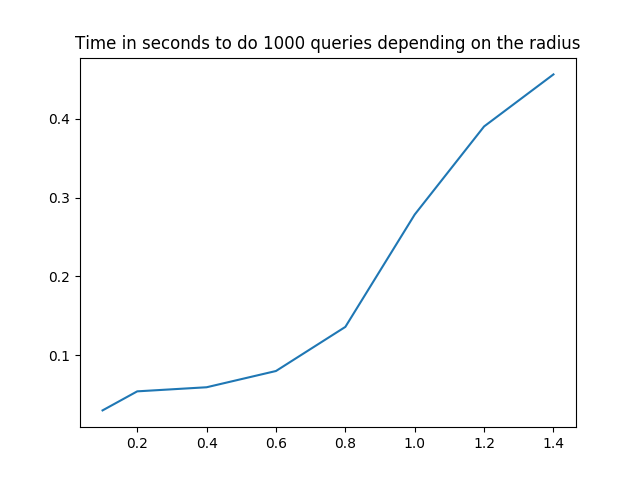
\includegraphics[width=0.6\linewidth]{kdt_radius.png}
	\caption{Évolution du temps en secondes nécessaire à 1000 recherches en fonction du rayon en mètres.}
	\label{fig:radius}
\end{figure}

\paragraph{Question 5.}
La Figure \ref{fig:q5} présente un même nuage dont la taille a été réduite par décimation ou selon une grille. La décimation est quasiment instantanée et est donc beaucoup plus rapide que la méthode par grille qui à pris environ 19 secondes. Toutefois le résultat obtenu à l'aide de la méthode par grille a une densité de points qui est plus régulière : il n'y a pas de trous dans le nuage.


\begin{figure}[h]
	\centering
	\begin{minipage}{0.47\linewidth}
		\centering
		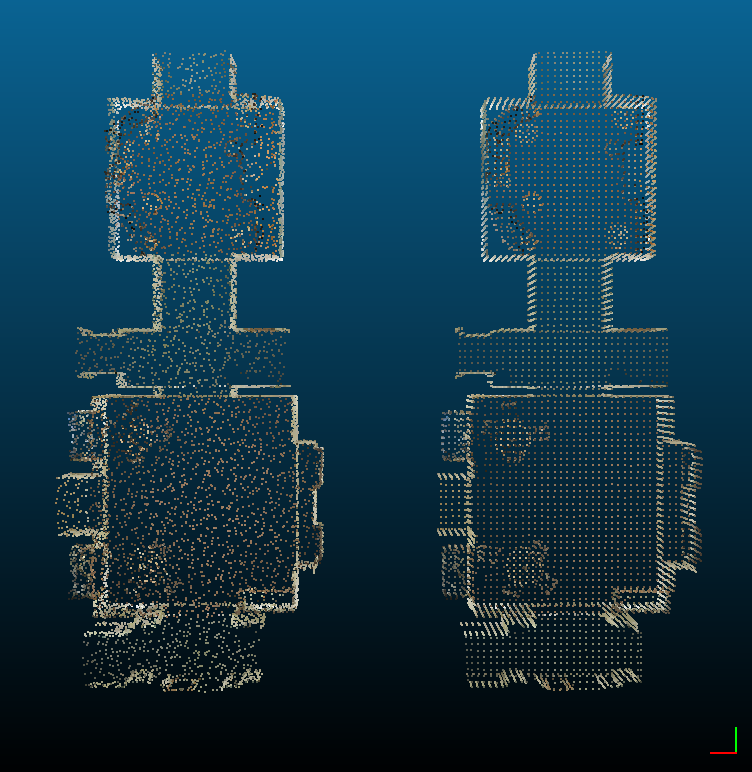
\includegraphics[width=\linewidth]{q5-1.png}
	\end{minipage}\hfill
	\begin{minipage}{0.47\linewidth}
		\centering
		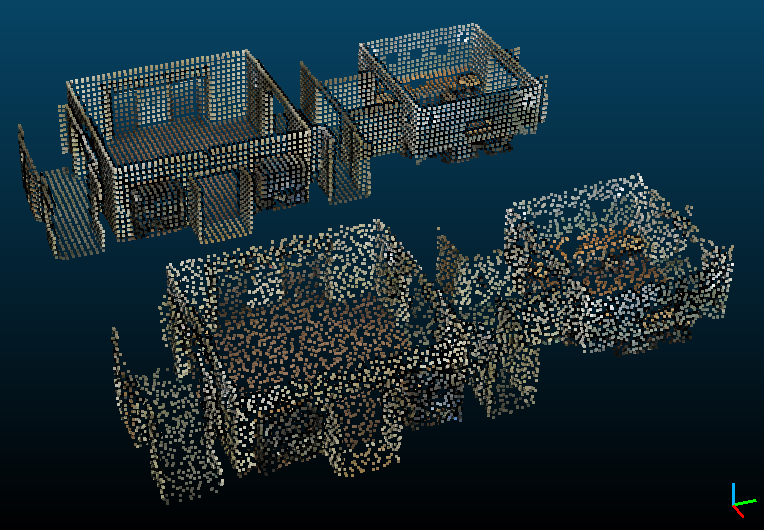
\includegraphics[width=\linewidth]{q5-2.png}
	\end{minipage}
	\caption{Vue du nuage après décimation et après échantillonnage sur grille (à droite sur l'image de gauche et au fond sur l'image de droite).}
	\label{fig:q5}
\end{figure}

\paragraph{Question bonus.}
La Figure \ref{fig:qbonus} montre le nuage de points avec étiquettes obtenu après réduction par grille.

\begin{figure}[h]
	\centering
	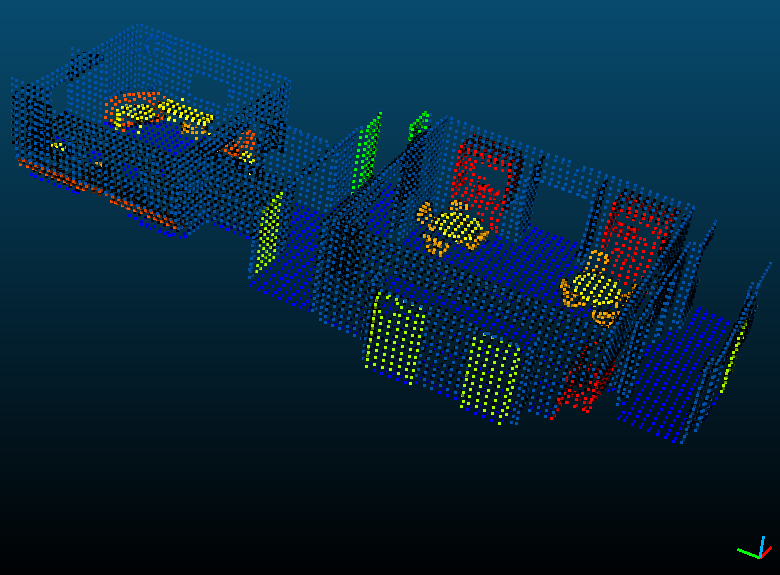
\includegraphics[width=0.6\linewidth]{qb1.png}
	\caption{Nuage de points avec étiquettes réduit à l'aide de la méthode de la grille.}
	\label{fig:qbonus}
\end{figure}

\end{document}
